\documentclass[a4paper,man,natbib,floatsintext,12pt]{apa7}

\usepackage[english]{babel} %character and hyphenation rules specific to the language you choose
%\usepackage[utf8x]{inputenc}
\usepackage{graphicx}
\usepackage{color}
\usepackage{tikz}
\usepackage{amsmath}
\usepackage{blindtext}
\usepackage{tabularx} %great for APA-style Tables
\usepackage{siunitx} % Required for good table alignmen
\sisetup{
  round-mode          = places, % Rounds numbers
  round-precision     = 2, % to 2 places
}
\usepackage{multirow}
\usepackage{booktabs}
\usepackage{wrapfig}
\usetikzlibrary{shapes,decorations,arrows,calc,arrows.meta,fit,positioning}
\tikzset{
    -Latex,auto,node distance =1 cm and 1 cm,semithick,
    latent/.style ={ellipse, draw, minimum width = 0.7 cm},
    observed/.style ={rectangle, draw},
    bidirected/.style={Latex-Latex,dashed},
    el/.style = {inner sep=2pt, align=left, sloped}
}
\newcommand{\sigFtest}[4]{\textit{F}(#1,#2) = #3, \textit{p}$<$#4}
\newcommand{\nonsigFtest}[3]{\textit{F}(#1,#2) = #3, \textit{p}$>$.05}


\title{My First Manuscript in \LaTeX  }
\shorttitle{This is the short title}
\author{Paul D. Kieffaber}
\affiliation{College of William \& Mary}
\journal{The Best Psychology Journal EVER!}
\abstract{\blindtext}
\keywords{APA style, demonstration}
\authornote{I would like to thank my dogs for sitting quietly while I worked on this.}
\leftheader{Alternate page header in man mode}

%-------------- END PREAMBLE  -------------------


\begin{document}

\maketitle  %Insert my APA style title page

\section{Introduction}

Your introduction goes here.  You might talk about previous work on cognitive deficits in schizophrenia \citep{brenner2014role}. Or you might want to explain how you used the Student \citet{student1908probable} \textit{t} distribution and present the formula you used to do significance testing for a correlation (see equation \ref{eq1}).
\begin{equation} \label{eq1}
t=\frac{r_{xy} \sqrt{n-2}}{ \sqrt{1-r^{2}_{xy}}}
\end{equation}

\blindtext


\section{Method}

Your method goes here!
\subsection{Participants}
Information about your participants goes here!
\subsection{Materials and Procedure}
Information about the details of your experiment goes here!

\section{Results}

A repeated measures 2 x 3 between-within ANOVA was conducted to assess changes in FAD behaviors over time and determine if the PNF for FAD condition demonstrates the most significant effects (see Table~\ref{tab:study}). Additionally, a mediation analysis was be conducted to examine whether FAD norms mediate the relationship between intervention type and FAD behaviors.

An a priori power analysis was conducted to determine the required sample size to detect a small effect size for a repeated-measures ANOVA (within-between interaction) using G*Power 3.1. It was decided to use a small effect size (f = 0.10) to be conservative, as no previous PNF interventions for FAD could be used as a reference. Past research indicated a small-moderate effect size of PNF interventions for alcohol use and problems (Dotson et al., 2015; Young \& Neighbors, 2019). The analysis was based on an alpha level of 0.05 and a desired power of 0.80. There were two groups (i.e., PNF-FAD, and control) and three measurement points (i.e., baseline, two-week and four-week follow-ups). The analysis indicated a minimum sample size of 164 participants per condition with these parameters to detect a statistically significant effect. Additionally, one research article suggests that a sample size of at least 562 participants is required to detect small effects in a partial mediation model with 0.80 power (Fritz \& Mackinnon, 2007). The goal was to recruit 650 participants to account for potential dropout rates.

\begin{table}[h!]
\centering
\caption{\label{tab:study}Engagement in FAD behaviors in the experimental and control groups. 0 = Never, 6 = Always.}
\begin{tabular}{l l c c c}
 \toprule
                          &              & \multicolumn{3}{c}{Study}\\
  \cmidrule{3-5}
                          &              & {Baseline}           & {Time 2}           & {Time 3}\\
  \cmidrule{3-5}
  \multirow{ 2}{*}{Group} & Experimental &     1.25    &      1.06     &      1.01     \\
                          & Control      &     1.23      &      1.67     &      1.23   \\
  \bottomrule
 \end{tabular}
\end{table}


\begin{figure}[ht!]
\centering
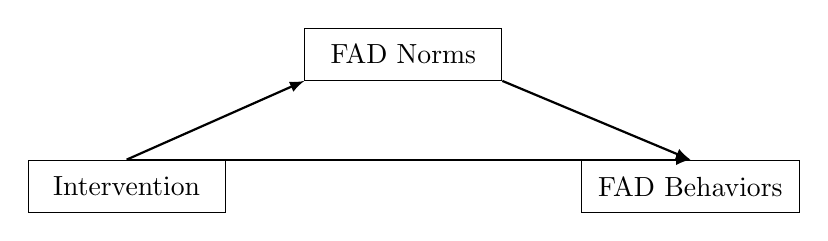
\begin{tikzpicture}[
  mynode/.style={draw, align=center, minimum width=2.5cm, inner sep=6pt}
]

% Nodes
\node[mynode] (M) {FAD Norms};
\node[mynode, below left=of M] (A) {Intervention};
\node[mynode, below right=of M] (B) {FAD Behaviors};

% Paths (only indirect mediation)
\draw[-latex, thick] (A.north) -- (M.south west);
\draw[-latex, thick] (M.south east) -- (B.north);
\draw[-latex, thick] (A.north) -- (B.north);

\end{tikzpicture}
\caption{\label{fig:TikZmodel}Mediation model of intervention effects on changes in FAD behaviors through changes in perceived FAD norms.}
\end{figure}

\section{Discussion}
Because the Discussion section will often refer back to the results, it is useful to take advantage of cross-referencing (see Table~\ref{tab:RTmeans}). 

Sometimes the discussion section may even include additional figures.  If the figures are small enough and you don't want them to take up the full line, you can always use the \texttt{wrapfigure} environment.

\begin{wrapfigure}{l}{0.4\textwidth}     \centering       
\includegraphics[width=0.25\textwidth]{brain-lateral.png}
\caption{\label{fig:latbrain} Yet another figure caption here.}
\end{wrapfigure}

Figure~\ref{fig:gearhead} was also a great example for the Results right? But what if you have a small figure and you just want to wrap the text neatly around it?  Never fear....the ``wrapfig'' package is here! The wrapfig environment allows you to neatly wrap text around your figures just like the journals do. \blindtext



\bibliography{references.bib}

\end{document}
https://www.overleaf.com/project/64ef8e5b3faa92d4248ddcf9